%------------------------------------------------------------------------------
\begin{frame}
    \frametitle{Problem Definition}
    2D square plate of side 1 m with one hot side and other 3 cold sides
    \begin{figure}
        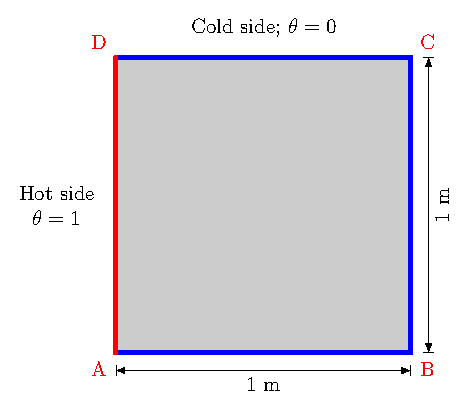
\includegraphics[scale=0.7]{00_schematic/01_problem_schematic/problemDefinition.pdf}
    \end{figure}

    Present work is to compute the temperature field within plate domain
    using PINNs with different variations in methodology.
\end{frame}

%------------------------------------------------------------------------------
\begin{frame}
    \frametitle{Governing equation and Analytical solution}

    \begin{figure}
        \centering
        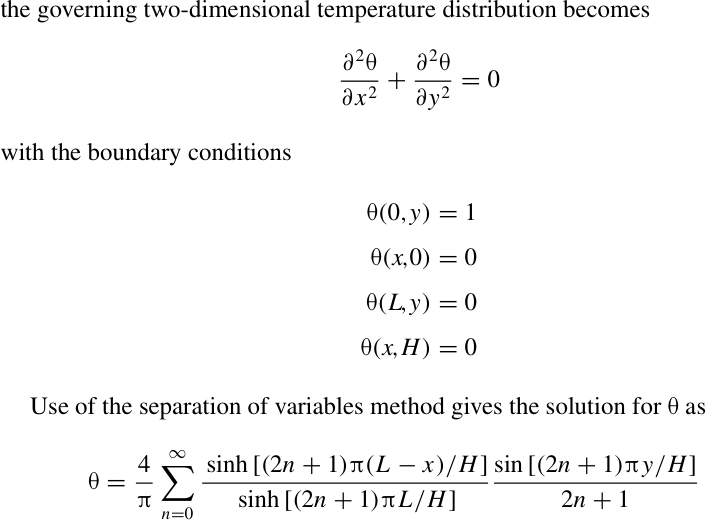
\includegraphics[scale=0.4]{supportingFiles/eqn.png}
    \end{figure}
\end{frame}

%------------------------------------------------------------------------------

\begin{frame}
    \frametitle{Network Schematic}
    \begin{figure}
        \centering
        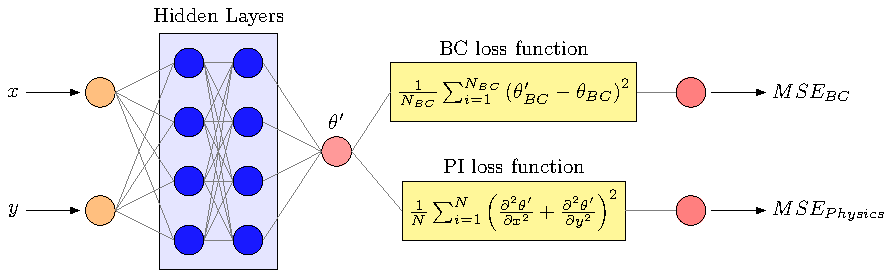
\includegraphics[scale=0.77]{00_schematic/02_PINN_schematic/PINN_HC_schematic.pdf}
    \end{figure}
\end{frame}

%------------------------------------------------------------------------------

\begin{frame}
    \frametitle{key points}

    \begin{itemize}
        \item pure physics-based training was done on the network with 20NX8L size,
            with 40 boundary points and 100 internal points.
            \vspace{1cm}
        \item the model was trained with 40,000 epochs and took about 3 minutes.
            Then the model is used to predict the solution on a 1 million grid.
            \vspace{1cm}
        \item The grid-extended solution was compared with analytical solution,
            the numerical solution was attempted for the same grid using FDM on
            FORTRAN with Gauss-seidel method.
    \end{itemize}
\end{frame}

%------------------------------------------------------------------------------

\begin{frame}
    \frametitle{Run-time comparison: PINN vs FDM}
    On 1 million grid,
    \begin{itemize}
        \item PINN took 172.42 seconds (2.87 minutes), including training time
        \item FDM took 1635.79 seconds (27.63 minutes)
    \end{itemize}
    \begin{columns}

        \begin{column}{0.5\textwidth}
            \begin{figure}
                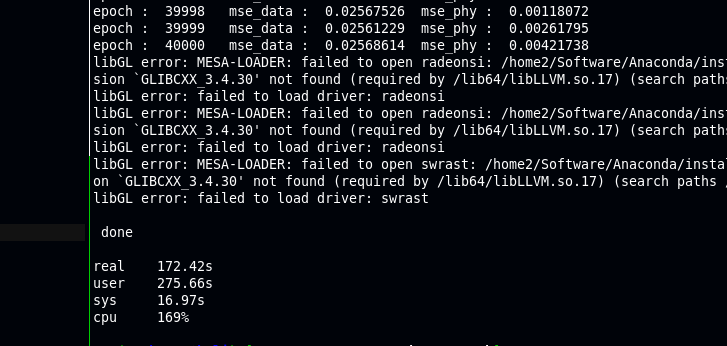
\includegraphics[scale=0.3]{supportingFiles/runtime_PINN.png}
                \caption{PINN runtime}
            \end{figure}
        \end{column}

        \begin{column}{0.5\textwidth}
            \begin{figure}
                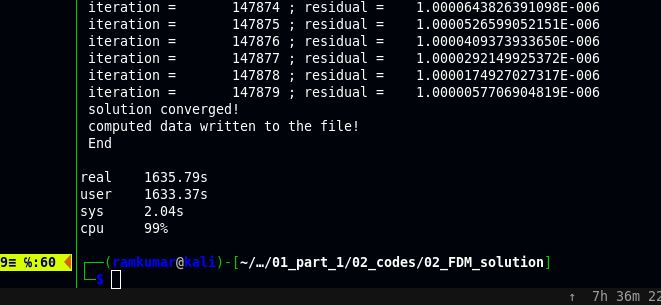
\includegraphics[scale=0.3]{supportingFiles/runtime_FDM.png}
                \caption{PINN runtime}
            \end{figure}
        \end{column}

    \end{columns}
\end{frame}

%------------------------------------------------------------------------------

\begin{frame}
    \frametitle{Solution Comparison: PINN vs Analytical : 1 Mil grid}
    \begin{figure}
        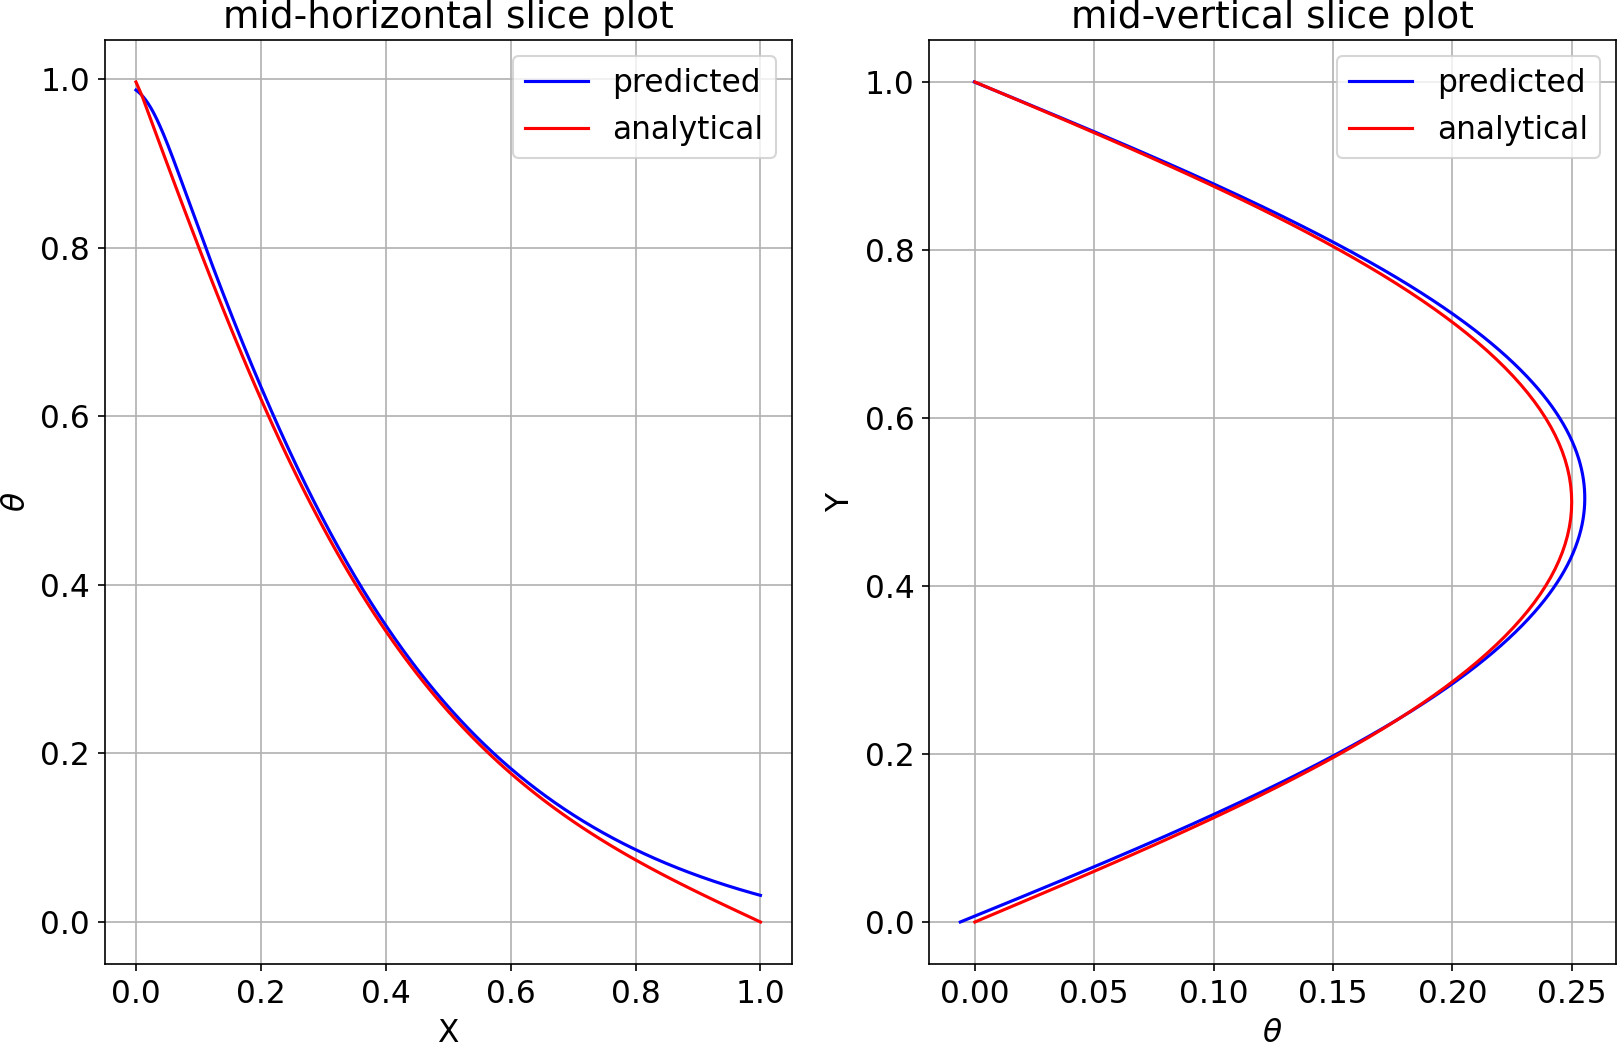
\includegraphics[scale=0.4]{supportingFiles/slice_plots_out.png}
    \end{figure}
\end{frame}

\begin{frame}
    \frametitle{Solution Comparison: PINN vs Analytical : 1 Mil grid}
    \begin{figure}
        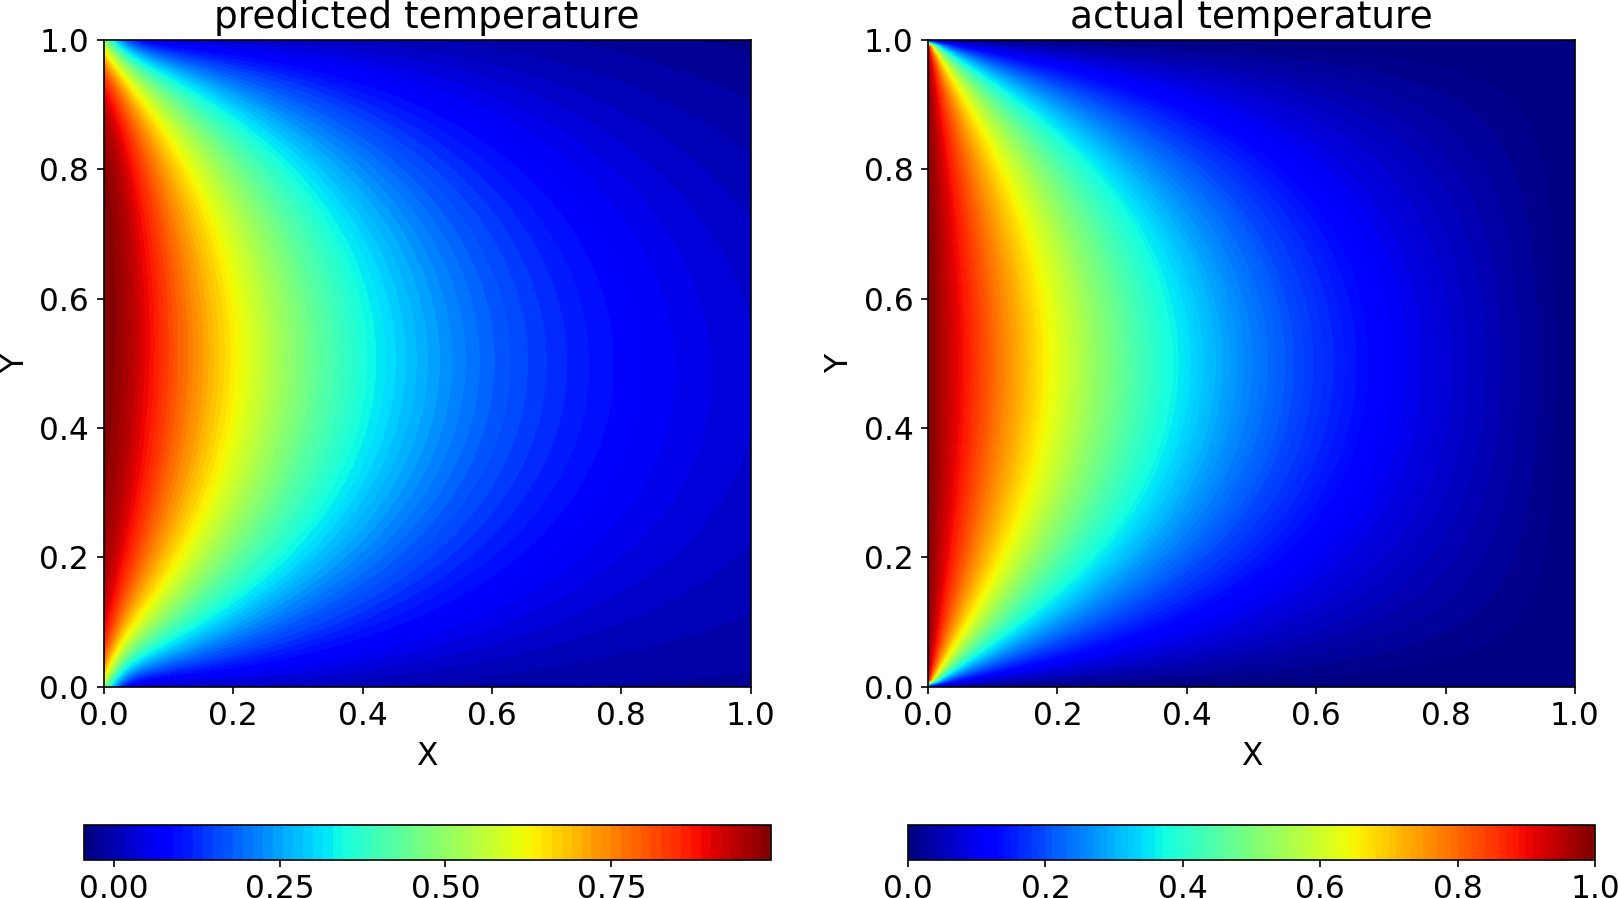
\includegraphics[scale=0.4]{supportingFiles/contours_out.png}
    \end{figure}
\end{frame}

%------------------------------------------------------------------------------

\begin{frame}
    \frametitle{Solution Comparison: FDM vs Analytical : 1 Mil grid}
    \begin{figure}
        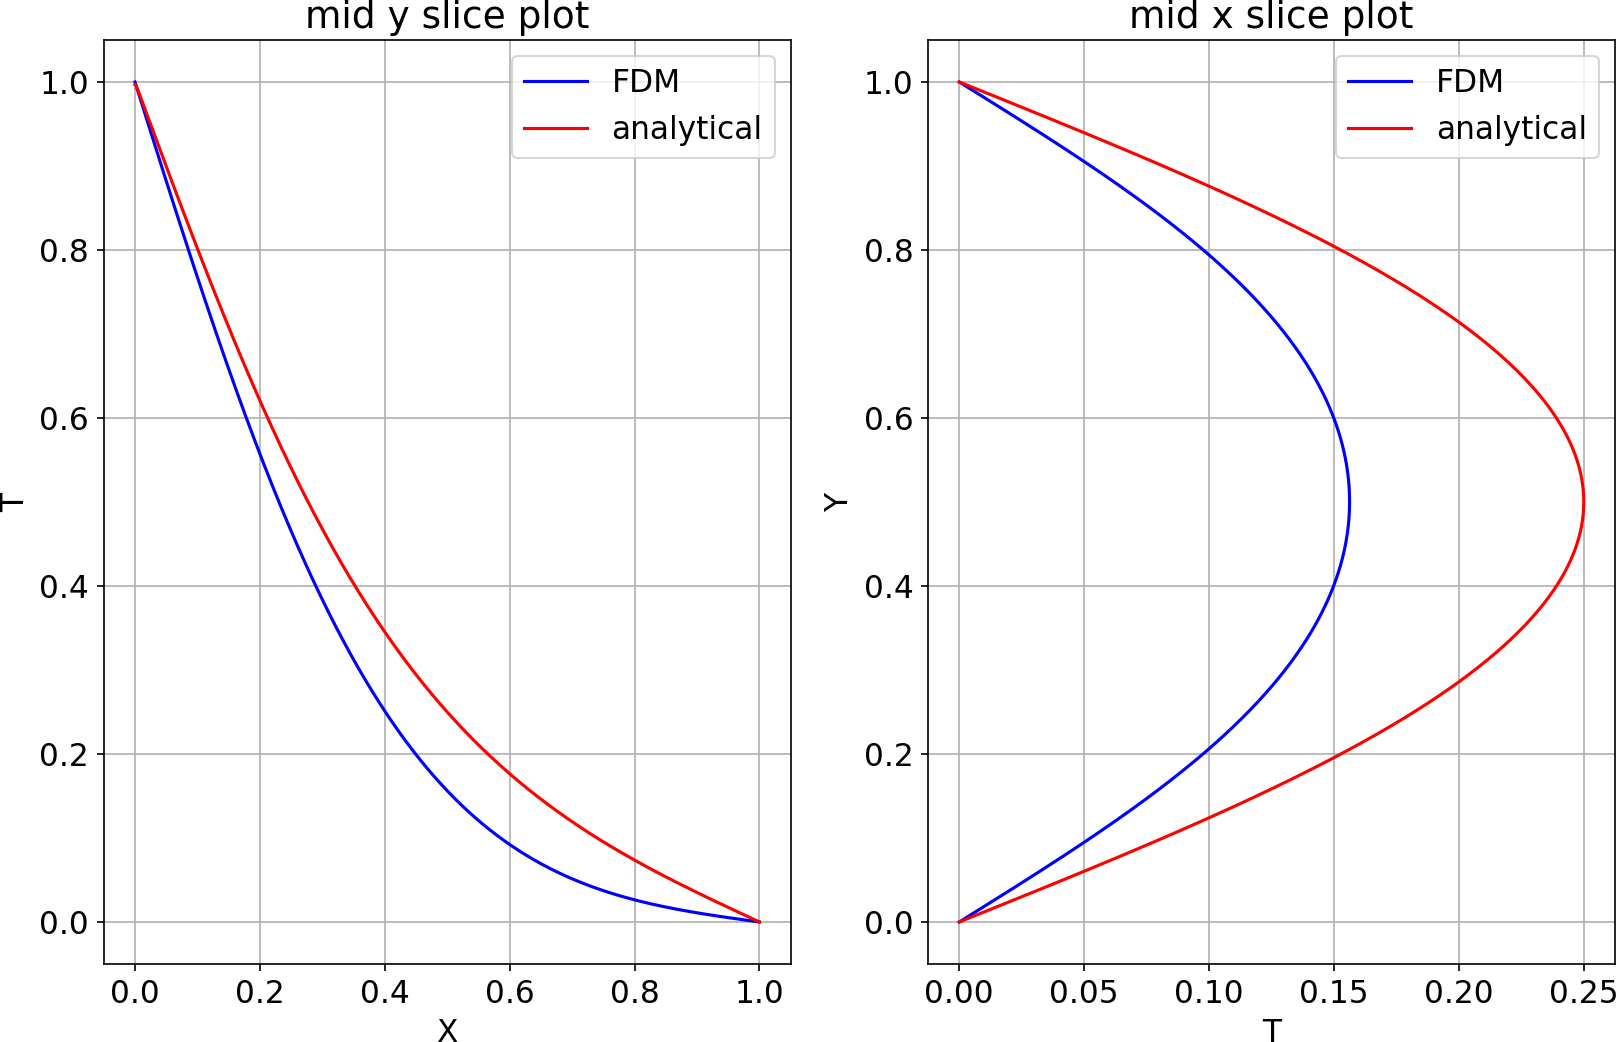
\includegraphics[scale=0.4]{supportingFiles/plots_FDM.png}
    \end{figure}
\end{frame}

%------------------------------------------------------------------------------

\begin{frame}
    \frametitle{Conclusion}
    \begin{enumerate}
        \item FDM solution did not match with analytical solution despite its
            convergence.
            \vspace{0.5cm}
        \item PINN's grid-extended solution matches with analytical solution.
            \vspace{0.5cm}
        \item PINN learns the function quite well by solving the problem with
            just 140 data points in the domain.
            \vspace{0.5cm}
        \item The time taken by PINN is 10 times less than FDM for the same
            grid solution, including training time.
            \vspace{0.5cm}
        \item PINN solution can be used as initial condition for steady state
            problems on large grids to save computational time.
    \end{enumerate}
\end{frame}
